\section{Results} 
\label{sec:6_results}
This section presents the empirical findings from our evaluation of the proposed probabilistic AI models and benchmarks for financial time series forecasting. We first analyze the predicted distributions, including shape and dynamics. 
%We begin by visualizing and summarizing the predicted return distributions, including key statistics such as skewness and kurtosis. 
We then evaluate distributional accuracy and calibration of these distributions using aforementioned methodology. Tail risk estimation is then assessed through both Value-at-Risk (VaR) and, with greater emphasis, Expected Shortfall (ES), using backtesting procedures and accuracy scoring rules. Finally, we disentangle and analyze aleatoric and epistemic uncertainty in the models' predictive distributions.
% ==================== Model Output ==================== %
\subsection{Model Output}
\label{sec:results_model_output}

The proposed models produce daily, one-step-ahead forecasts of full conditional return distributions for each stock in the dataset. 
%, including predicted means, standard deviations, mixture components, and associated weights—all of which are dynamically updated daily based on new information. 
These are expressed as mixtures of Gaussian components, defined by time-varying parameters: predictive means, variances, mixture weights, and component structures. All components are dynamically updated in response to new data, reflecting the conditional evolution of market states.

Figures \ref{fig:descriptive_analysis_of_AAPL_daily_returns} and \ref{fig:descriptive_analysis_of_WMT_daily_returns} illustrate examples of these predictive distributions for Apple (AAPL) and Walmart (WMT) on two distinct dates. The presented dates are selected programmatically at random, ensuring an unbiased representation of the models' predictive capabilities rather than optimized or handpicked outcomes. The distributions, visualized as mixtures of Gaussian components weighted by the model, clearly deviate from normality, reflecting pronounced heavy-tailed characteristics consistent with findings from the Jarque-Bera diagnostic tests. Furthermore, skewness and excess kurtosis statistics indicate notable asymmetry and leptokurtosis in the predictive distributions, emphasizing the models' flexibility in capturing complex return dynamics. Importantly, the predictive distributions exhibit day-to-day variability, observable in changes in mean, variance, mixture composition, and component weights, demonstrating the models' conditional adaptability to evolving market conditions. Additionally, differences between assets are apparent; AAPL consistently exhibits more extreme predictions compared to WMT on the same dates, aligning with market perceptions of greater volatility typically associated with technology stocks relative to retail stocks (REFERENCE). These observations underscore the capability of the proposed models to capture both temporal variability and cross-sectional differences in return distributions.

\begin{figure}[H]
    \centering
    \begin{subfigure}[b]{0.49\textwidth}
        \centering
        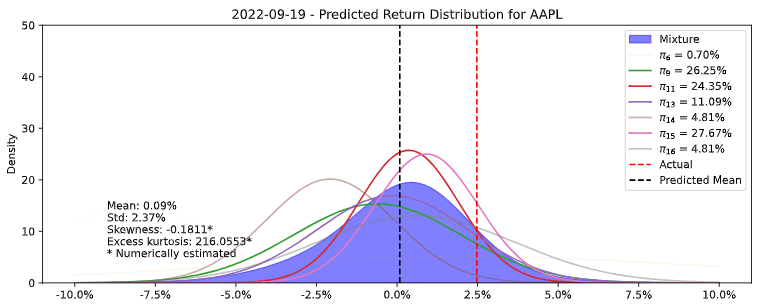
\includegraphics[width=\linewidth, height=5cm]{Images/Results/APPL_distribution_example_1.png}
        \caption{Predicted return distribution for AAPL on 2022-09-19, showing a slightly right-skewed distribution with multiple mixture components.}
        \label{fig:APPL_distribution_example_1}
    \end{subfigure}
    \hfill
    \begin{subfigure}[b]{0.49\textwidth}
        \centering
        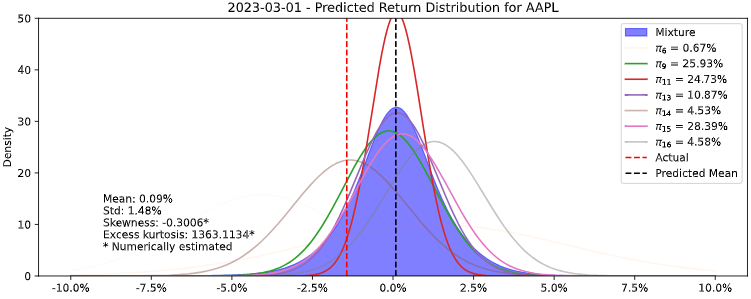
\includegraphics[width=\linewidth, height=5cm]{Images/Results/APPL_distribution_example_2.png}
        \caption{Predicted return distribution for AAPL on 2023-03-01, showing a peaked distribution with heavier tails.}
        \label{fig:APPL_distribution_example_2}
    \end{subfigure}
    \caption{Distribution of predicted return for APPL}
    \label{fig:descriptive_analysis_of_AAPL_daily_returns}
\end{figure}  

\begin{figure}[H]
    \centering
    \begin{subfigure}[b]{0.49\textwidth}
        \centering
        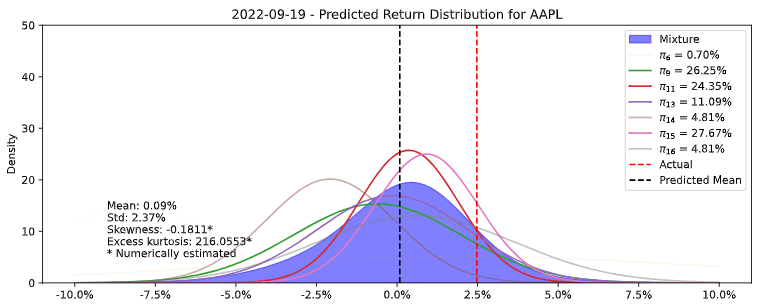
\includegraphics[width=\linewidth, height=5cm]{Images/Results/APPL_distribution_example_1.png}
        \caption{Predicted return distribution for WMT on 2022-09-19, ... }
        \label{fig:WMT_distribution_example_1}
    \end{subfigure}
    \hfill
    \begin{subfigure}[b]{0.49\textwidth}
        \centering
        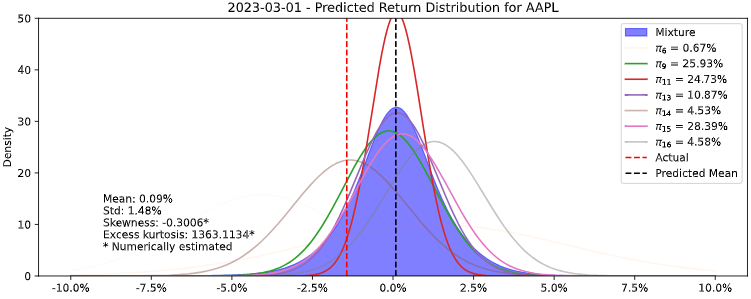
\includegraphics[width=\linewidth, height=5cm]{Images/Results/APPL_distribution_example_2.png}
        \caption{Predicted return distribution for WMT on 2022-09-19, ....}
        \label{fig:WMT_distribution_example_2}
    \end{subfigure}

    \caption{Distribution of predicted return for WMT}
    \label{fig:descriptive_analysis_of_WMT_daily_returns}
\end{figure}

Figures \ref{fig:weight_evolution_mixtures} further illustrates the evolution of mixture component weights over time for AAPL and WMT, demonstrating the adaptive capability of the proposed models. Notably, the allocation of weights across the mixture components differs between the two assets, confirming that the model tailors its distributional representations to asset-specific characteristics. Although the temporal variation in component weights appears moderate, subtle fluctuations indicate the model's sensitivity in dynamically adjusting to shifting market conditions. However, the relatively stable patterns suggest that, once trained, the model captures persistent structural characteristics within each asset’s return distribution, requiring only incremental adjustments over short horizons. This ability to maintain structural consistency while flexibly adapting to changing market nuances constitutes a strength, as it balances complexity with stability in probabilistic forecasts.

\begin{figure}[H]
    \centering
    \begin{subfigure}[b]{0.49\textwidth}
        \centering
        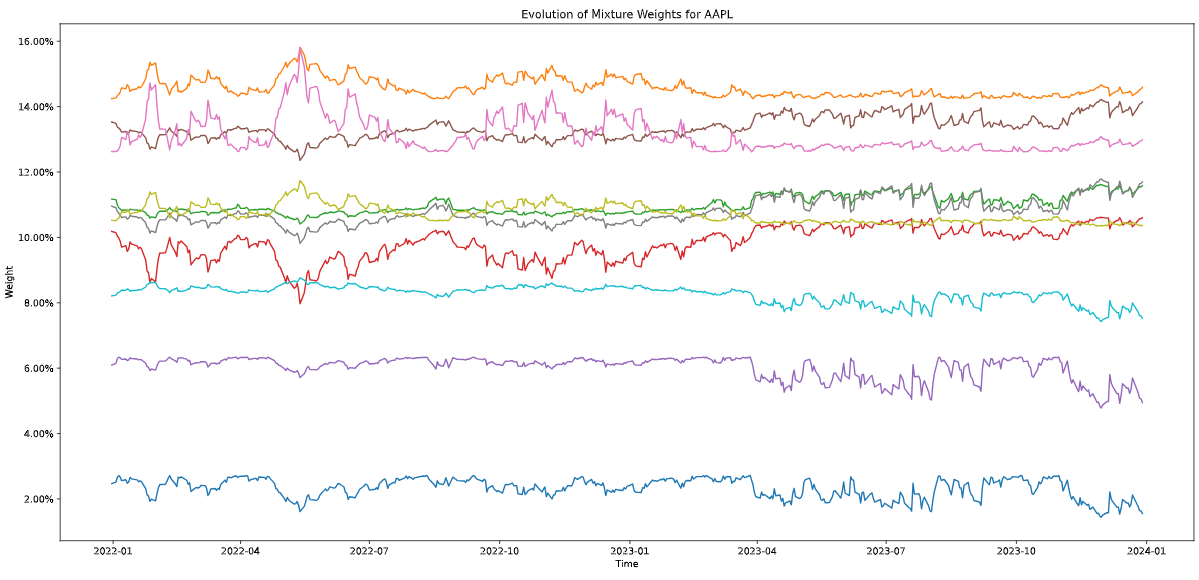
\includegraphics[width=\linewidth, height=5cm]{Images/Results/APPL_weight_evolution_mixtures.png}
        \caption{Time-series of estimated mixture component weights for AAPL, showing relatively stable component contributions over time}
        \label{fig:APPL_weight_evolution_mixtures}
    \end{subfigure}
    \hfill
    \begin{subfigure}[b]{0.49\textwidth}
        \centering
        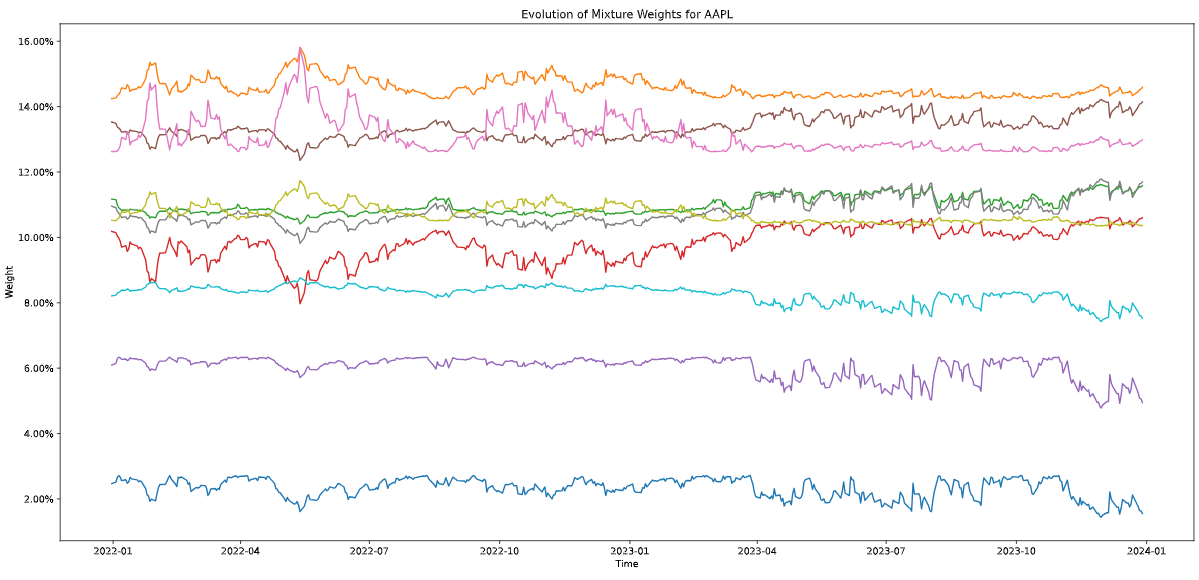
\includegraphics[width=\linewidth, height=5cm]{Images/Results/APPL_weight_evolution_mixtures.png}
        \caption{Time-series of estimated mixture component weights for WMT, ...}
        \label{fig:WMT_weight_evolution_mixtures}
    \end{subfigure}
    \caption{Temporal evolution of mixture component weights for AAPL and WMT}
    \label{fig:weight_evolution_mixtures}
\end{figure}

Lastly, Figure \ref{fig:time_series_roilling_prediction_150_days} displays the predicted return distributions for the final 150 days of the test dataset for AAPL and WMT, segmented by different confidence intervals. Notably, the predicted mean returns remain consistently near zero over this period, closely aligning with the observed average realized returns, demonstrating that the models stick to the central tendency of returns. However, the predicted distributions exhibit clear variability over time and differ substantially between the two assets, emphasizing the models' capacity to dynamically adapt to asset-specific volatility structures and market conditions. Furthermore, the illustrated confidence intervals highlight that the model distributions successfully encompass most actual returns within one standard deviation (the 67\% interval), indicating good calibration. Additionally, more extreme return outcomes are mostly captured by higher confidence intervals.

\begin{figure}[H]
    \centering
    \begin{subfigure}[b]{0.49\textwidth}
        \centering
        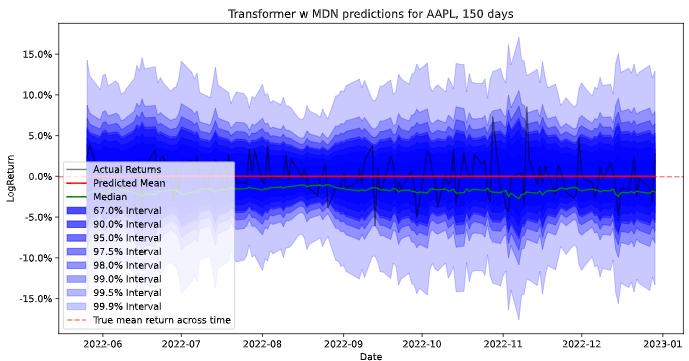
\includegraphics[width=\linewidth, height=5cm]{Images/Results/APPL_time_series_example_1.png}
        \caption{Rolling predicted return distributions for APPL with 5\% to 95\% confidence intervals.}
        \label{fig:APPL_time_series_example_150_days}
    \end{subfigure}
    \hfill
    \begin{subfigure}[b]{0.49\textwidth}
        \centering
        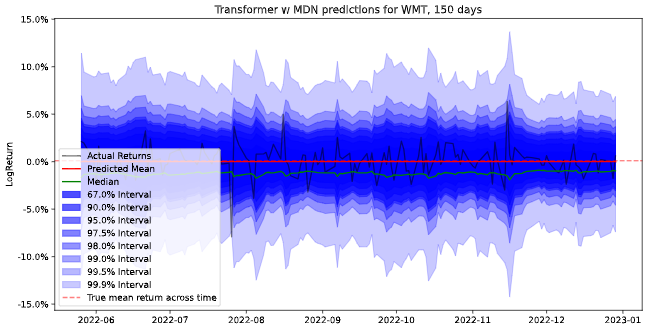
\includegraphics[width=\linewidth, height=5cm]{Images/Results/WMT_time_series_example_1.png}
        \caption{Rolling predicted return distributions for WMT with 5\% to 95\% confidence intervals.}
        \label{fig:WMT_time_series_example_150_days}
    \end{subfigure}
    \caption{Time-series of rolling one-day-ahead predicted return distributions (150-day horizon).}
    \label{fig:time_series_roilling_prediction_150_days}
\end{figure}

SHOW COMPARISON GRAPH WITH GARCH!!!!!!!!!!!!!

%Table \ref{table:forecast_moments} .... excess kurtosis ... [WRITE SOMETHING HERE]

% \begin{table}[H]
%     \centering
%     \caption[Moments of Forecasted Distributions Across Models]{Moments of Forecasted Distributions Across Models}
%     \label{table:forecast_moments}
%     \begin{adjustbox}{width=1\textwidth,center}
%     \begin{tabular}{p{0.3\textwidth}p{0.175\textwidth}p{0.175\textwidth}p{0.175\textwidth}p{0.175\textwidth}}
%         \toprule
%         \textbf{Model} &\textbf{Mean} & \textbf{Variance} & \textbf{Skewness} & \textbf{Excess Kurtosis} \\
%         \midrule
%         \multicolumn{5}{l}{\textbf{Proposed Models}} \\
%         LSTM-MDN-RV  & x & x & x & x \\
%         LSTM-MDN-IV  & x & x & x & x \\
%         LSTM-MDN-RV-IV  & x & x & x & x \\
%         Transformer-MDN-RV  & x & x & x & x \\
%         Transformer-MDN-IV  & x & x & x & x \\
%         Transformer-MDN-RV-IV  & x & x & x & x \\
%         \addlinespace
%         \hdashline[0.2pt/3pt]
%         \addlinespace
%         \multicolumn{5}{l}{\textbf{Traditional Benchmarks}} \\
%         GARCH & x & x & x & x \\
%         GARCH-t & x & x & x & x \\
%         EGARCH & x & x & x & x \\
%         RV-GARCH & x & x & x & x \\
%         AR-GARCH & x & x & x & x \\
%         AR-GARCH-t & x & x & x & x \\
%         HAR & x & x & x & x \\
%         HARQ & x & x & x & x \\
%         DB-RV & x & x & x & x \\ 
%         DB-IV & x & x & x & x \\
%         DB-RV-IV & x & x & x & x \\
%         \addlinespace
%         \hdashline[0.2pt/3pt]
%         \addlinespace
%         \multicolumn{5}{l}{\textbf{Machine Learning Benchmarks}} \\
%         XgBoost-RV  & x & x & x & x \\
%         XgBoost-IV  & x & x & x & x \\
%         XgBoost-RV-IV  & x & x & x & x \\
%         CatBoost-RV  & x & x & x & x \\
%         CatBoost-IV  & x & x & x & x \\
%         CatBoost-RV-IV  & x & x & x & x \\
%         LigthGBM-RV  & x & x & x & x \\
%         LigthGBM-IV  & x & x & x & x \\
%         LigthGBM-RV-IV  & x & x & x & x \\
%         \bottomrule
%     \end{tabular}   
%     \end{adjustbox}
% \end{table}  


% ==================== Distribution Accuracy ==================== %
\subsection{Distribution Accuracy}
\label{sec:distribution_accuracy}

To assess distributional accuracy regarding predictive precision, calibration, and coverage, we evaluate the models' performance using Negative Log-Likelihood (NLL), Expected Calibration Error (ECE), Continuous Ranked Probability Score (CRPS), and Prediction Interval Coverage Probability (PICP) across multiple confidence levels (REFERENCE). Table \ref{table:distribution_accuracy_and_picp} summarizes these scores, with the best-performing model for each metric highlighted in bold. Lower NNL and CRPS scores indicated more precise and concentrated predictive distributions, while low ECE value confirm accurate calibration. From these results, the proposed models generally exhibit favorable performance compared to benchmark models. 
Prediction interval coverage is also well aligned with nominal levels, across all intervals, where most of the proposed models achieve near-ideal coverage.


\begin{table}[H]
    \centering
    \caption[Distribution Accuracy and Calibration Metrics]{Distribution Accuracy and Calibration Metrics}
    \label{table:distribution_accuracy_and_picp}
    \begin{adjustbox}{width=\textwidth,center}
    \begin{tabular}{
        p{0.25\textwidth}
        >{\centering\arraybackslash}p{0.1\textwidth}
        >{\centering\arraybackslash}p{0.1\textwidth}
        >{\centering\arraybackslash}p{0.1\textwidth}
        @{\hspace{3em}}
        >{\centering\arraybackslash}p{0.1\textwidth}
        >{\centering\arraybackslash}p{0.1\textwidth}
        >{\centering\arraybackslash}p{0.1\textwidth}
        >{\centering\arraybackslash}p{0.1\textwidth}
    }
        \toprule
        \textbf{Model} & \textbf{NLL} & \textbf{ECE} & \textbf{CRPS} 
        & \multicolumn{4}{c}{\textbf{PICP}} \\
        \cmidrule(lr){5-8}
        & & & & 67\% & 90\% & 95\% & 98\% \\
        \midrule
        \multicolumn{4}{l}{\textbf{Proposed Models}} \\
        LSTM-MDN-RV & \textbf{-2.9534} & \textbf{0.0206} & \textbf{0.0037} & 65.82\% & \textbf{89.51\%} & 94.47\% & 97.78\% \\
        LSTM-MDN-IV & \textbf{-2.9653} & \textbf{\underline{0.0057}} & \textbf{0.0038} & 65.05\% & 88.99\% & 94.23\% & 97.56\% \\
        LSTM-MDN-RV-IV & \textbf{-2.9645} & \textbf{0.0197} & \textbf{\underline{0.0036}} & \textbf{67.83\%} & \textbf{\underline{89.94\%}} & 94.84\% & 97.96\% \\
        Transformer-MDN-RV & \textbf{-2.9582} & \textbf{0.0080} & \textbf{0.0041} & \textbf{\underline{66.63\%}} & \textbf{89.72\%} & 94.64\% & 97.68\% \\
        Transformer-MDN-IV & \textbf{-2.9589} & \textbf{0.0077} & \textbf{0.0041} & 65.16\% & 88.81\% & 93.88\% & 97.59\% \\
        Transformer-MDN-RV-IV & \textbf{-2.9674} & \textbf{0.0077} & \textbf{0.0039} & 65.87\% & 89.20\% & 94.30\% & 97.64\% \\
        \addlinespace
        \hdashline[0.2pt/3pt]
        \addlinespace
        \multicolumn{4}{l}{\textbf{Traditional Benchmarks}} \\
        GARCH & -2.8595 & 0.0376 & 0.0066 & 76.64\% & 92.84\% & 95.73\% & 97.54\% \\
        GARCH-t & -2.8819 & 0.0468 & 0.0076 & 79.67\% & 95.73\% & 97.98\% & 99.10\% \\
        EGARCH & -2.8658 & 0.0364 & 0.0066 & 76.41\% & 92.76\% & 95.81\% & 97.51\% \\
        RV-GARCH & -2.8580 & 0.0344 & 0.0065 & 75.70\% & 92.27\% & 95.48\% & 97.24\% \\
        AR-GARCH & -2.8599 & 0.0374 & 0.0066 & 76.62\% & 92.82\% & 95.70\% & 97.52\% \\
        AR-GARCH-t & -2.8826 & 0.0466 & 0.0076 & 79.75\% & 95.72\% & 97.93\% & 99.10\% \\
        HAR & -2.3843 & 0.0695 & 0.0059 & 47.54\% & 70.51\% & 78.14\% & 84.37\% \\
        HARQ & -2.3916 & 0.0692 & 0.0059 & 47.48\% & 70.64\% & 78.29\% & 84.50\% \\
        DB-RV & - & - & - & - & - & - \\
        DB-IV & - & - & - & - & - & - \\
        DB-RV-IV & - & - & - & - & - & - \\
        \addlinespace
        \hdashline[0.2pt/3pt]
        \addlinespace
        \multicolumn{4}{l}{\textbf{Machine Learning Benchmarks}} \\
        XgBoost-RV & - & - & - & 68.98\% & 91.25\% & 95.53\% & 98.34\% \\
        XgBoost-IV & - & - & - & 68.47\% & 90.82\% & 95.25\% & 98.04\% \\
        XgBoost-RV-IV & - & - & - & 67.92\% & 90.79\% & 95.23\% & 98.15\% \\
        CatBoost-RV & - & - & - & 68.95\% & 91.27\% & 95.63\% & 98.26\% \\
        CatBoost-IV & - & - & - & 68.31\% & 90.66\% & \underline{95.05\%} & 97.80\% \\
        CatBoost-RV-IV & - & - & - & 67.95\% & 90.60\% & 94.90\% & 97.78\% \\
        LigthGBM-RV & - & - & - & 68.94\% & 91.25\% & 95.61\% & 98.21\% \\
        LigthGBM-IV & - & - & - & 68.21\% & 90.94\% & 95.14\% & 98.12\% \\
        LigthGBM-RV-IV & - & - & - & 68.03\% & 90.68\% & 94.91\% & \underline{98.02\%} \\
        \bottomrule
    \end{tabular}
    \end{adjustbox}
    \par\vspace{0.3em} % Forces space between table and footnote
    {\raggedright\footnotesize{Note: \textbf{Bold} indicates better performance than Traditional and ML benchmarks. \underline{Underscore} indicates the best performing model.}}
\end{table}

Additionally, Table \ref{table:model_confidence_set_distributional_accuracy_by_coverage} presents the outcomes of the Model Confidence Set (MCS) analysis at the 75\% and 90\% significance levels, identifying subsets of statistically indistinguishable top-performing models. The analysis consistently places our proposed models within these top-performing subsets, suggesting robust and competitive predictive capabilities. Although certain benchmarks cannot be statistically differentiated from our models across all metrics based on MCS results, the frequent inclusion of the proposed models in the optimal subsets indicates their effectiveness in capturing accurate and calibrated distributional forecasts.  

\begin{table}[H]
    \centering
    \caption[Model Confidence Set (MCS) — Distribution Accuracy]{Model Confidence Set (MCS) — Distribution Accuracy}
    \label{table:model_confidence_set_distributional_accuracy_by_coverage}
    \begin{adjustbox}{width=1\textwidth,center}
    \begin{tabular}{
        p{0.28\textwidth}  % Model column
        >{\centering\arraybackslash}p{0.12\textwidth}
        >{\centering\arraybackslash}p{0.12\textwidth}
        >{\centering\arraybackslash}p{0.12\textwidth}
        >{\centering\arraybackslash}p{0.12\textwidth}
        >{\centering\arraybackslash}p{0.12\textwidth}
        >{\centering\arraybackslash}p{0.12\textwidth}
    }
        \toprule
        \textbf{Model} 
        & \multicolumn{3}{c}{\textbf{75\% confidence level}} 
        & \multicolumn{3}{c}{\textbf{95\% conficence level}} \\
        \cmidrule(lr){2-4} \cmidrule(lr){5-7}
        & NLL & CRPS & Performance
        & NLL & CRPS & Performance \\
        \midrule
        \multicolumn{7}{l}{\textbf{Proposed Models}} \\
        LSTM-MDN-RV &   &   & 0 &   &   & 0 \\
        LSTM-MDN-IV & \checkmark &   & 50 & \checkmark &   & 50 \\
        LSTM-MDN-RV-IV & \checkmark & \checkmark & 100 & \checkmark & \checkmark & 100 \\
        Transformer-MDN-RV &   &   & 0 &   &   & 0 \\
        Transformer-MDN-IV &   &   & 0 &   &   & 0 \\
        Transformer-MDN-RV-IV & \checkmark &   & 50 & \checkmark &   & 50 \\
        \addlinespace
        \hdashline[0.2pt/3pt]
        \addlinespace
        \multicolumn{7}{l}{\textbf{Traditional Benchmarks}} \\
        GARCH &   &   & 0 &   &   & 0 \\
        GARCH-t &   &   & 0 &   &   & 0 \\
        EGARCH &   &   & 0 &   &   & 0 \\
        RV-GARCH &   &   & 0 &   &   & 0 \\
        AR-GARCH &   &   & 0 &   &   & 0 \\
        AR-GARCH-t &   &   & 0 &   &   & 0 \\
        HAR &   &   & 0 &   &   & 0 \\
        HARQ &   &   & 0 &   &   & 0 \\
        DB-RV & - & - & - & - & - & - \\
        DB-IV & - & - & - & - & - & - \\
        DB-RV-IV & - & - & - & - & - & - \\
        \bottomrule
    \end{tabular}
    \end{adjustbox}
\end{table}







% ==================== VaR Adequacy and Accuracy ==================== %
\subsection{VaR Adequacy and Accuracy}
\label{sec:var_adequacy_and_accuracy}

Although Expected Shortfall (ES) is the primary tail risk measure of interest in this study, we report Value-at-Risk (VaR) results across different quantiles to provide a more comprehensive evaluation of model performance.  We evaluate both the adequacy and accuracy of VaR predictions across the 95\%, 97.5\%, and 99\% quantiles.
 
We assess VaR adequacy using Christoffernsen Conditional Coverage test. Table \ref{table:var_adequacy_christoffersens_test} summarizes outcomes from the Christoffersen test for adequacy at the 95\%, 97.5\%, and 99\% quantiles. Given the multi-asset nature of our dataset, adequacy is assessed through the fail-rate approach recommended by Bayer \& Dimitriadis (REFERENCE), who state that an adequate model should exhibit a fail rate approximately equal to the significance level (p-value) used in the Christoffersen test. However, with the relatively small cross-sectional sample of 30 stocks, caution is necessary as isolated asset-level outcomes might disproportionately affect overall conclusions. Nevertheless, this asset-level adequacy assessment remains the best way to assess adequacy, as each stock represents a distinct return distribution. The results indicate that the proposed models generally achieve fail rates closely aligned with the respective test significance levels, suggesting that they are adequately capturing tail risks across all examined quantiles. This consistency supports the reliability of the proposed models for VaR estimation.

\begin{table}[H]
    \centering
    \caption[VaR Adequacy via Christoffersen Tests]{VaR Adequacy via Christoffersen Tests}
    \caption*{\small\textit{Number of passing and failing stocks in Christoffersen's Conditional Coverage test for VaR adequacy.}}

    \label{table:var_adequacy_christoffersens_test}
    \begin{adjustbox}{width=1\textwidth,center}
    \begin{tabular}{
        p{0.24\textwidth}
        >{\centering\arraybackslash}p{0.03\textwidth}
        >{\centering\arraybackslash}p{0.03\textwidth}
        >{\centering\arraybackslash}p{0.1\textwidth}
        >{\centering\arraybackslash}p{0.1\textwidth}
        >{\centering\arraybackslash}p{0.03\textwidth}
        >{\centering\arraybackslash}p{0.03\textwidth}
        >{\centering\arraybackslash}p{0.1\textwidth}
        >{\centering\arraybackslash}p{0.1\textwidth}
        >{\centering\arraybackslash}p{0.03\textwidth}
        >{\centering\arraybackslash}p{0.03\textwidth}
        >{\centering\arraybackslash}p{0.1\textwidth}
        >{\centering\arraybackslash}p{0.1\textwidth}
    }
        \toprule
        \textbf{Model} & \multicolumn{4}{c}{\textbf{95\% VaR}} & \multicolumn{4}{c}{\textbf{97.5\% VaR}} & \multicolumn{4}{c}{\textbf{99\% VaR}} \\
        \cmidrule(lr){2-5} \cmidrule(lr){6-9} \cmidrule(lr){10-13}
        & Pass & Fail & Inconclusive &  Fail Rate 
        & Pass & Fail & Inconclusive &  Fail Rate 
        & Pass & Fail & Inconclusive &  Fail Rate \\
        \midrule
        \multicolumn{13}{l}{\textbf{Proposed Models}} \\
        LSTM-MDN-RV & 22 & 6 & 1 & 21.4\% & 15 & 4 & 10 & 21.1\% & 4 & 0 & 25 & 0.0\% \\
        LSTM-MDN-IV & 20 & 8 & 1 & 28.6\% & 19 & 3 & 7 & 13.6\% & 6 & 1 & 22 & 14.3\% \\
        LSTM-MDN-RV-IV & 25 & 2 & 2 & 7.4\% & 17 & 1 & 11 & 5.6\% & 2 & 0 & 27 & 0.0\% \\
        Transformer-MDN-RV & 25 & 3 & 1 & 10.7\% & 18 & 2 & 9 & 10.0\% & 5 & 0 & 24 & 0.0\% \\
        Transformer-MDN-IV & 22 & 7 & 0 & 24.1\% & 17 & 4 & 8 & 19.0\% & 6 & 2 & 21 & 25.0\% \\
        Transformer-MDN-RV-IV & 26 & 3 & 0 & 10.3\% & 17 & 3 & 9 & 15.0\% & 5 & 1 & 23 & 16.7\% \\
        
        \addlinespace
        \hdashline[0.2pt/3pt]
        \addlinespace
        \multicolumn{13}{l}{\textbf{Traditional Benchmarks}} \\
        GARCH & 16 & 7 & 6 & 30.4\% & 13 & 1 & 15 & 7.1\% & 5 & 0 & 24 & 0.0\% \\
        GARCH-t & 1 & 12 & 16 & 92.3\% & 2 & 0 & 27 & 0.0\% & 0 & 0 & 29 & 0.0\% \\
        EGARCH & 15 & 11 & 3 & 42.3\% & 14 & 1 & 14 & 6.7\% & 6 & 1 & 22 & 14.3\% \\
        RV-GARCH & 18 & 8 & 3 & 30.8\% & 13 & 2 & 14 & 13.3\% & 7 & 0 & 22 & 0.0\% \\
        AR-GARCH & 17 & 8 & 4 & 32.0\% & 14 & 0 & 15 & 0.0\% & 5 & 0 & 24 & 0.0\% \\
        AR-GARCH-t & 1 & 12 & 16 & 92.3\% & 2 & 0 & 27 & 0.0\% & 0 & 0 & 29 & 0.0\% \\
        HAR & 0 & 29 & 0 & 100.0\% & 0 & 29 & 0 & 100.0\% & 0 & 29 & 0 & 100.0\% \\
        HARQ & 0 & 29 & 0 & 100.0\% & 0 & 29 & 0 & 100.0\% & 0 & 29 & 0 & 100.0\% \\
        DB-RV & - & - & - & - & - & - & - & - & - & - & - & - \\
        DB-IV & - & - & - & - & - & - & - & - & - & - & - & - \\
        DB-RV-IV & - & - & - & - & - & - & - & - & - & - & - & - \\
        \addlinespace
        \hdashline[0.2pt/3pt]
        \addlinespace
        \multicolumn{13}{l}{\textbf{Machine Learning Benchmarks}} \\
        XgBoost-RV & 20 & 5 & 4 & 20.0\% & 9 & 4 & 16 & 30.8\% & 1 & 0 & 28 & 0.0\% \\
        XgBoost-IV & 24 & 4 & 1 & 14.3\% & 14 & 4 & 11 & 22.2\% & 2 & 1 & 26 & 33.3\% \\
        XgBoost-RV-IV & 23 & 5 & 1 & 17.9\% & 13 & 2 & 14 & 13.3\% & 2 & 0 & 27 & 0.0\% \\
        CatBoost-RV & - & - & - & -& - & - & - & -& - & - & - & -\\
        CatBoost-IV & 25 & 3 & 1 & 10.7\% & 13 & 4 & 12 & 23.5\% & 3 & 1 & 25 & 25.0\% \\
        CatBoost-RV-IV & 22 & 5 & 2 & 18.5\% & 12 & 3 & 14 & 20.0\% & 2 & 1 & 26 & 33.3\% \\
        LigthGBM-RV & 19 & 7 & 3 & 26.9\% & 8 & 2 & 19 & 20.0\% & 1 & 0 & 28 & 0.0\% \\
        LigthGBM-IV & 22 & 5 & 2 & 18.5\% & 12 & 4 & 13 & 25.0\% & 3 & 2 & 24 & 40.0\% \\
        LigthGBM-RV-IV & 24 & 3 & 2 & 11.1\% & 11 & 5 & 13 & 31.2\% & 4 & 1 & 24 & 20.0\% \\
        \bottomrule
    \end{tabular}
    \end{adjustbox}
\end{table}

VaR accuracy is evaluated with interval score and mean width. These metric are only interpretable for adequate models (REFERNCE). Nevertheless, we report them for all models for comparison. Table \ref{table:var_accuracy_interval_score_mean_width} presents the results. Lower values indicate better performance, and bold representing best performing model among adequate models. Among the adequate models, the proposed architectures achieves significant lower interval score and mean width, in indicating a more efficient tail risk estimation, without overestimation risk. 

\begin{table}[H]
    \centering
    \caption[Interval Score and Mean Width (VaR Forecasts)]{Interval Score and Mean Width (VaR Forecasts)}
    \label{table:var_accuracy_interval_score_mean_width}
    \begin{adjustbox}{width=1\textwidth,center}
    \begin{tabular}{
        p{0.25\textwidth}
        >{\centering\arraybackslash}p{0.125\textwidth}
        >{\centering\arraybackslash}p{0.125\textwidth}
        >{\centering\arraybackslash}p{0.125\textwidth}
        >{\centering\arraybackslash}p{0.125\textwidth}
        >{\centering\arraybackslash}p{0.125\textwidth}
        >{\centering\arraybackslash}p{0.125\textwidth}
    }
        \toprule
        \textbf{Model} 
        & \multicolumn{2}{c}{\textbf{95\% VaR}} 
        & \multicolumn{2}{c}{\textbf{97.5\% VaR}} 
        & \multicolumn{2}{c}{\textbf{99\% VaR}} \\
        \cmidrule(lr){2-3} \cmidrule(lr){4-5} \cmidrule(lr){6-7}
        & Interval Score & Mean Width & Interval Score & Mean Width & Interval Score & Mean Width \\
        \midrule
        \multicolumn{7}{l}{\textbf{Proposed Models}} \\
        LSTM-MDN-RV & \textbf{0.0435} & \textbf{0.0412} & \textbf{0.0533} & \textbf{0.0520} & \textbf{0.0689} & \textbf{0.0682} \\
        LSTM-MDN-IV & \textbf{0.0438} & \textbf{0.0417} & \textbf{0.0538} & \textbf{0.0527} & \textbf{0.0688} & \textbf{0.0684} \\
        LSTM-MDN-RV-IV & \textbf{0.0449} & \textbf{0.0429} & \textbf{0.0549} & \textbf{0.0538} & 0.0702 & 0.0697 \\
        Transformer-MDN-RV & \textbf{\underline{0.0436}} & \textbf{\underline{0.0414}} & \textbf{0.0532} & \textbf{\underline{0.0519}} & \textbf{0.0680} & \textbf{0.0673} \\
        Transformer-MDN-IV & \textbf{0.0441} & \textbf{0.0419} & \textbf{0.0536} & \textbf{0.0525} & \textbf{0.0679} & \textbf{0.0673} \\
        Transformer-MDN-RV-IV & \textbf{0.0436} & \textbf{0.0415} & \textbf{\underline{0.0532}} & \textbf{0.0521} & \textbf{\underline{0.0675}} & \textbf{\underline{0.0670}} \\
        
        \addlinespace
        \hdashline[0.2pt/3pt]
        \addlinespace
        \multicolumn{7}{l}{\textbf{Traditional Benchmarks}} \\
        GARCH & 0.0511 & 0.0493 & 0.0599 & 0.0588 & 0.0705 & 0.0698 \\
        GARCH-t & 0.0604 & 0.0592 & 0.0761 & 0.0754 & 0.0989 & 0.0986 \\
        EGARCH & 0.0506 & 0.0488 & 0.0593 & 0.0582 & 0.0698 & 0.0691 \\
        RV-GARCH & 0.0504 & 0.0486 & 0.0590 & 0.0579 & 0.0695 & 0.0687 \\
        AR-GARCH & 0.0510 & 0.0493 & 0.0598 & 0.0587 & 0.0704 & 0.0697 \\
        AR-GARCH-t & 0.0603 & 0.0592 & 0.0760 & 0.0754 & 0.0989 & 0.0985 \\
        HAR* & 0.0307 & 0.0249 & 0.0339 & 0.0297 & 0.0383 & 0.0353 \\
        HARQ* & 0.0308 & 0.0250 & 0.0340 & 0.0298 & 0.0383 & 0.0353 \\
        DB-RV & - & - & - & - & - & - \\
        DB-IV & - & - & - & - & - & - \\
        DB-RV-IV & - & - & - & - & - & - \\
        \bottomrule
    \end{tabular} 
    \end{adjustbox}
    \par\vspace{0.3em} % Forces space between table and footnote
    {\raggedright\footnotesize{Note: \textbf{Bold} indicates better performance than all Traditional Benchmarks. \underline{Underscore} indicates the best performing model. \\ * Model is clearly inadequate and is thus not marked as the winner despite the score being superior.}\par}
\end{table}



% ==================== ES Adequacy and Accuracy ==================== %
\subsection{ES Adequacy and Accuracy}
\label{sec:es_adequacy_and_accuracy} 

%- Short about Bayer-Dimitriadis repetition, why we look at fail rate
%- Comment on what models can be considered adequate
%- Comment on why we look at the two significance levels --> to get more robust interpretation, and robustness is key in tail risk, so it makes sense


We further evaluate the tail risk through Expected Shortfall (ES) which accounts for the magnitude of extreme losses beyond VaR thresholds. Since ES cannot be directly backtested directly using coverage tests, we adopt the conditional calibration approach introduced by \textcite{Bayer2020}, extended to 95\%, 97.5\% and 99\% levels to examine performance and statistical consistency with realized returns at different levels of tail risk. The adequacy test is performed at both 1\% and 5\% significance levels to enhance the robustness of our findings, making it possible to distinguish those model who are marginally adequate and constituently reliable. Table \ref{table:es_adequacy_Bayer_dimitriadis_test} shows the failrate of Bayer-Dimitriadis test for the stocks at both 1\% and 5\% significance level. A lower fail rate indicates stronger statistical adequacy.

Our proposed models demonstrate adequacy in modeling tail risk, with several architectures passing the Beyer-Dimitriadis test at the 95\% and 99\% guantile levels. in particular, the Transformer-MDN-RV-IV achieve the lowest fail rate across models, with fail rate as low as 3.5\% and 6.9\%. Notably, many ML bechmarks also demonstrate strong adequacy. Due to the limited number of violations in the 99\% levels, we are not able to produce and report results for this quantile from adequacy evaluation for any model. 

\begin{table}[H]
    \centering
    \caption[ES Adequacy via Bayer-Dimitriadis Test]{ES Adequacy via Bayer-Dimitriadis Test}
    \caption*{\small\textit{Number of passing and failing stocks in Bayer-Dimitriadis test for ES adequacy.}}
    \label{table:es_adequacy_Bayer_dimitriadis_test}
    \begin{adjustbox}{width=1\textwidth,center}
    \begin{tabular}{
        p{0.3\textwidth} % model
        >{\centering\arraybackslash}p{0.058\textwidth}
        >{\centering\arraybackslash}p{0.058\textwidth}
        >{\centering\arraybackslash}p{0.117\textwidth}
        >{\centering\arraybackslash}p{0.058\textwidth}
        >{\centering\arraybackslash}p{0.058\textwidth}
        >{\centering\arraybackslash}p{0.117\textwidth}
        >{\centering\arraybackslash}p{0.058\textwidth}
        >{\centering\arraybackslash}p{0.058\textwidth}
        >{\centering\arraybackslash}p{0.117\textwidth}
    }
        \toprule
        \textbf{Model} 
        & \multicolumn{3}{c}{\textbf{95\% ES}} 
        & \multicolumn{3}{c}{\textbf{97.5\% ES}} 
        & \multicolumn{3}{c}{\textbf{99\% ES}} \\
        \cmidrule(lr){2-4} \cmidrule(lr){5-7} \cmidrule(lr){8-10}
        & Pass & Fail & Fail Rate 
        & Pass & Fail & Fail Rate 
        & Pass & Fail & Fail Rate \\
        \midrule
        
        \multicolumn{10}{l}{\textbf{Proposed Models}} \\
        LSTM-MDN-RV & 26 & 3 & 10.34\% & 26 & 3 & 10.34\% & 0 & 0 & N/A \\
        LSTM-MDN-IV & 25 & 4 & 13.79\% & 25 & 4 & 13.79\% & 0 & 0 & N/A \\
        LSTM-MDN-RV-IV & 27 & 2 & 6.90\% & 25 & 4 & 13.79\% & 0 & 0 & N/A \\
        Transformer-MDN-RV & 19 & 10 & 34.48\% & 15 & 14 & 48.28\% & 0 & 0 & N/A \\
        Transformer-MDN-IV & 25 & 4 & 13.79\% & 26 & 3 & 10.34\% & 0 & 0 & N/A \\
        Transformer-MDN-RV-IV & 28 & 1 & 3.45\% & 26 & 2 & 6.90 \% & 0 & 0 & N/A \\
        
        \addlinespace
        \hdashline[0.2pt/3pt]
        \addlinespace
        
        \multicolumn{10}{l}{\textbf{Traditional Benchmarks}} \\
        GARCH & 17 & 5 & 22.73\% & 20 & 2 & 9.09\% & 0 & 0 & N/A \\
        GARCH-t & 5 & 24 & 82.76\% & 11 & 18 & 62.07\% & 0 & 0 & N/A \\
        EGARCH & 19 & 3 & 13.64\% & 22 & 0 & 0.00\% & 0 & 0 & N/A \\
        RV-GARCH & 22 & 7 & 24.14\% & 27 & 2 & 6.90\% & 0 & 0 & N/A \\
        AR-GARCH & 21 & 8 & 27.59\% & 27 & 2 & 6.90\% & 0 & 0 & N/A \\
        AR-GARCH-t & - & - & - & - & - & - & - & - & - \\ % not in origiN/Al table
        HAR & 1 & 28 & 96.55\% & 5 & 24 & 82.76\% & 0 & 0 & N/A \\
        HARQ & 0 & 29 & 100.00\% & 5 & 24 & 82.76\% & 0 & 0 & N/A \\
        DB-RV & 26 & 3 & 10.34\% & 26 & 3 & 10.34\% & 0 & 0 & N/A \\
        DB-IV & 27 & 2 & 6.90\% & 25 & 4 & 13.79\% & 0 & 0 & N/A \\
        DB-RV-IV & 28 & 1 & 3.45\% & 26 & 3 & 10.34\% & 0 & 0 & N/A \\
        
        \addlinespace
        \hdashline[0.2pt/3pt]
        \addlinespace
        
        \multicolumn{10}{l}{\textbf{Machine Learning Benchmarks}} \\
        XgBoost-RV & 26 & 3 & 10.34\% & 27 & 2 & 6.90\% & 0 & 0 & N/A \\
        XgBoost-IV & - & - & - & - & - & - & - & - & - \\ % not in original table
        XgBoost-RV-IV & - & - & - & - & - & - & - & - & - \\ % not in original table
        CatBoost-RV & - & - & - & - & - & - & - & - & - \\ % not in original table
        CatBoost-IV & 27 & 2 & 6.90\% & 25 & 4 & 13.79\% & 0 & 0 & N/A \\
        CatBoost-RV-IV & 29 & 0 & 0.00\% & 27 & 2 & 6.90\% & 0 & 0 & N/A \\
        LigthGBM-RV & 26 & 3 & 10.34\% & 27 & 2 & 6.90\% & 0 & 0 & N/A \\
        LigthGBM-IV & 27 & 2 & 6.90\% & 28 & 1 & 3.45\% & 0 & 0 & N/A \\
        LigthGBM-RV-IV & 28 & 1 & 3.45\% & 27 & 2 & 6.90\% & 0 & 0 & N/A \\
        \bottomrule
    \end{tabular}
    \end{adjustbox}
\end{table}


To evaluate accuracy, we report Fissler-Ziegel (FZ) and Asymmetric Laplace (AL) scores in Table \ref{table:es_accuracy_fz_and_al_score}, which jointly assess the accuracy and calibration of VaR-ES forecast (REFERENCE?). Lower values indicate better performance. Across all quantiles, our proposed models consistently outperform traditional benchmarks, and match or excess the performance of the ML benchmarks. Notably, Transformer-MDN-RV-IV and LSTM-MDN-IV provides the strongest overall results, with Transformer-MDN-RV-IV achieving lowest FZ and Al score for 95\% level, and LSTM-MDN-IV performing best at the 97.5\% and 99\% levels. 


\begin{table}[H]
    \centering
    \caption[Fissler-Ziegel (FZ) and Asymmetric Laplace (AL) Scoring Rules for ES Accuracy]{Fissler-Ziegel (FZ) and Asymmetric Laplace (AL) Scoring Rules for ES Accuracy}
    \label{table:es_accuracy_fz_and_al_score}
    \begin{adjustbox}{width=1\textwidth,center}
    \begin{tabular}{
        p{0.3\textwidth}
        >{\centering\arraybackslash}p{0.11667\textwidth}
        >{\centering\arraybackslash}p{0.11667\textwidth}
        >{\centering\arraybackslash}p{0.11667\textwidth}
        >{\centering\arraybackslash}p{0.11667\textwidth}
        >{\centering\arraybackslash}p{0.11667\textwidth}
        >{\centering\arraybackslash}p{0.11667\textwidth}
    }
        \toprule
        \textbf{Model} & \multicolumn{2}{c}{\textbf{95\% Quantile}} & \multicolumn{2}{c}{\textbf{97.5\% Quantile}} & \multicolumn{2}{c}{\textbf{99\% Quantile}} \\
        \cmidrule(lr){2-3} \cmidrule(lr){4-5} \cmidrule(lr){6-7}
        & FZ-score & AL-score 
        & FZ-score & AL-score 
        & FZ-score & AL-score \\
        \midrule
        \multicolumn{7}{l}{\textbf{Proposed Models}} \\
        LSTM-MDN-RV &  -3.5100 &  -2.4366 &  -3.2923 &  -2.2491 &  -3.0257 &  -2.0019 \\
        LSTM-MDN-IV &  \textbf{-3.5441} &  \textbf{-2.4714} &  \underline{\textbf{-3.3507}} &  \underline{\textbf{-2.3078}} &  \underline{\textbf{-3.1328}} &  \underline{\textbf{-2.1089}} \\
        LSTM-MDN-RV-IV &  \textbf{-3.5425} &  \textbf{-2.4704} &  \textbf{-3.3461} &  \textbf{-2.3037} &  \textbf{-3.1146} &  \textbf{-2.0911} \\
        Transformer-MDN-RV &  -3.5049 &  -2.4342 &  -3.2743 &  -2.2343 &  -2.9630 &  -1.9433 \\
        Transformer-MDN-IV &  \textbf{-3.5355} &  \textbf{-2.4627} &  \textbf{-3.3400} &  \textbf{-2.2970} &  \textbf{-3.1168} &  \textbf{-2.0928} \\
        Transformer-MDN-RV-IV &  \underline{\textbf{-3.5449}} &  \underline{\textbf{-2.4720}} &  \textbf{-3.3479} &  \textbf{-2.3048} &  \textbf{-3.1178} &  \textbf{-2.0937} \\
        \addlinespace
        \hdashline[0.2pt/3pt]
        \addlinespace
        \multicolumn{7}{l}{\textbf{Traditional Benchmarks}} \\
        GARCH & -3.4491 & -2.3762 & -3.2290 & -2.1846 & -2.9089 & -1.8821 \\
        GARCH-t & -3.3728 & -2.3056 & -3.1517 & -2.1133 & -2.8812 & -1.8608 \\
        EGARCH & -3.4578 & -2.3851 & -3.2372 & -2.1930 & -2.9146 & -1.8879 \\
        RV-GARCH & -3.4452 & -2.3713 & -3.2156 & -2.1704 & -2.8753 & -1.8478 \\
        AR-GARCH & - & - & - & - & - & - \\
        AR-GARCH-t & - & - & - & - & - & - \\
        HAR & -2.8513 & -1.7501 & -2.1404 & -1.0711 & -0.6651 & 0.3836 \\
        HARQ & -2.8606 & -1.7595 & -2.1561 & -1.0869 & -0.6981 & 0.3504 \\
        DB-RV & - & - & - & - & - & - \\
        DB-IV & - & - & - & - & - & - \\
        DB-RV-IV & - & - & - & - & - & - \\
        \addlinespace
        \hdashline[0.2pt/3pt]
        \addlinespace
        \multicolumn{7}{l}{\textbf{Machine Learning Benchmarks}} \\
        XgBoost-RV & -3.4980 & -2.4227 & -3.2847 & -2.2400 & -3.0277 & -2.0026 \\
        XgBoost-IV & -3.5259 & -2.4519 & -3.3301 & -2.2861 & -3.0913 & -2.0660 \\
        XgBoost-RV-IV & -3.5284 & -2.4532 & -3.3217 & -2.2771 & -3.0874 & -2.0621 \\
        CatBoost-RV & - & -& - & -& - & -\\
        CatBoost-IV & -3.5346 & -2.4608 & -3.3363 & -2.2925 & -3.1080 & -2.0832 \\
        CatBoost-RV-IV & -3.5274 & -2.4518 & -3.3258 & -2.2811 & -3.0863 & -2.0611 \\
        LigthGBM-RV & -3.4941 & -2.4193 & -3.2850 & -2.2402 & -3.0268 & -2.0016 \\
        LigthGBM-IV & -3.5330 & -2.4587 & -3.3344 & -2.2902 & -3.1055 & -2.0805 \\
        LigthGBM-RV-IV & -3.5259 & -2.4509 & -3.3264 & -2.2817 & -3.0881 & -2.0626 \\
        \bottomrule
    \end{tabular}
    \end{adjustbox}
    \par\vspace{0.3em} % Forces space between table and footnote
    {\raggedright\footnotesize{Note: \textbf{Bold} indicates better performance than Traditional and ML benchmarks. \underline{Underscore} indicates the best performing model.}}
\end{table}


Table \ref{table:model_confidence_set_ES_accuracy_by_coverage} presents the Model Confidence Set results for ES accuracy. At both 75\% and 95\% confidence levels, our models — particularly LSTM-MDN-IV,  LSTM-MDN-RV-IV, Transformer-MDN-IV and Transformer-MDN-RV-IV— are consistently included in the set of statistically indistinguishable best-performing models—providing strong evidence for their significant superiority in tail risk modeling over traditional benchmark models. Traditional benchmarks are excluded entirely from the best-performing models. However, several ML benchmark models, including CatBoost-IV, XgBoost-RV-IV, and LightGBM-IV, show competitive performance and are frequently added in the confidence set. 

\begin{table}[H]
    \centering
    \caption[Inclusions in Model Confidence Set (MCS) across the three estimated quantiles (95\%, 97.5\%, 99\%) — ES Forecasts]{Model Confidence Set (MCS) — ES Forecasts}
    \label{table:model_confidence_set_ES_accuracy_by_coverage}
    \begin{adjustbox}{width=1\textwidth,center}
    \begin{tabular}{
        p{0.24\textwidth}  % Model column
        >{\centering\arraybackslash}p{0.06\textwidth}
        >{\centering\arraybackslash}p{0.06\textwidth}
        >{\centering\arraybackslash}p{0.06\textwidth}
        >{\centering\arraybackslash}p{0.06\textwidth}
        >{\centering\arraybackslash}p{0.06\textwidth}
        >{\centering\arraybackslash}p{0.06\textwidth}
        >{\centering\arraybackslash}p{0.06\textwidth}
        >{\centering\arraybackslash}p{0.06\textwidth}
        >{\centering\arraybackslash}p{0.06\textwidth}
        >{\centering\arraybackslash}p{0.06\textwidth}
        >{\centering\arraybackslash}p{0.06\textwidth}
        >{\centering\arraybackslash}p{0.06\textwidth}
        >{\centering\arraybackslash}p{0.06\textwidth}
        >{\centering\arraybackslash}p{0.06\textwidth}
    }
        \toprule
        \textbf{Model} 
        & \multicolumn{7}{c}{\textbf{75\% Confidence Level}} 
        & \multicolumn{7}{c}{\textbf{95\% Confidence Level}} \\
        \cmidrule(lr){2-8} \cmidrule(lr){9-15}
        & $FZ_{95\%}$ & $AL_{95\%}$ & $FZ_{97.5\%}$ & $AL_{97.5\%}$ & $FZ_{99\%}$ & $AL_{99\%}$ & Perf 
        & $FZ_{95\%}$ & $AL_{95\%}$ & $FZ_{97.5\%}$ & $AL_{97.5\%}$ & $FZ_{99\%}$ & $AL_{99\%}$ & Perf \\
        \midrule
        \multicolumn{7}{l}{\textbf{Proposed Models}} \\
        LSTM-MDN-RV & & & & & & & 0 & \checkmark & & & & & & 16 \\
        LSTM-MDN-IV & \checkmark & \checkmark & \checkmark & \checkmark & \checkmark & \checkmark & 100 & \checkmark & \checkmark & \checkmark & \checkmark & \checkmark & \checkmark & 100 \\
        LSTM-MDN-RV-IV & \checkmark & \checkmark & \checkmark & \checkmark & \checkmark & \checkmark & 100 & \checkmark & \checkmark & \checkmark & \checkmark & \checkmark & \checkmark & 100 \\
        Transformer-MDN-RV & & & & & & & 0 & & & & & & & 0 \\
        Transformer-MDN-IV & \checkmark & \checkmark & \checkmark & \checkmark & \checkmark & \checkmark & 100 & \checkmark & \checkmark & \checkmark & \checkmark & \checkmark & \checkmark & 100 \\
        Transformer-MDN-RV-IV & \checkmark & \checkmark & \checkmark & \checkmark & \checkmark & \checkmark & 100 & \checkmark & \checkmark & \checkmark & \checkmark & \checkmark & \checkmark & 100 \\
        
        \addlinespace
        \hdashline[0.2pt/3pt]
        \addlinespace
        \multicolumn{7}{l}{\textbf{Traditional Benchmarks}} \\
        GARCH & & & & & & & 0 & & & & & & & 0 \\
        GARCH-t & & & & & & & 0 & & & & & & & 0 \\
        EGARCH & & & & & & & 0 & & & & & & & 0 \\
        RV-GARCH & & & & & & & 0 & & & & & & & 0 \\
        AR-GARCH & & & & & & & 0 & & & & & & & 0 \\
        AR-GARCH-t & & & & & & & 0 & & & & & & & 0 \\
        HAR & & & & & & & 0 & & & & & & & 0 \\
        HARQ & & & & & & & 0 & & & & & & & 0 \\
        DB-RV & - & - & - & - & - & - & - & - & - & - & - & - & - & - \\
        DB-IV & - & - & - & - & - & - & - & - & - & - & - & - & - & - \\
        DB-RV-IV & - & - & - & - & - & - & - & - & - & - & - & - & - & - \\
        \addlinespace
        \hdashline[0.2pt/3pt]
        \addlinespace
        \multicolumn{7}{l}{\textbf{Machine Learning Benchmarks}} \\
        XgBoost-RV & & & & & & & 0 & & & & & & & 0 \\
        XgBoost-IV & & & & & & & 0 & \checkmark & & \checkmark & \checkmark & \checkmark & \checkmark & 83 \\
        XgBoost-RV-IV & & & & & & & 0 & \checkmark & \checkmark & \checkmark & \checkmark & \checkmark & \checkmark & 100 \\
        CatBoost-RV & & & & & & & 0 & & & & & & & 0 \\
        CatBoost-IV & \checkmark & \checkmark & \checkmark & \checkmark & \checkmark & \checkmark & 100 & \checkmark & \checkmark & \checkmark & \checkmark & \checkmark & \checkmark & 100 \\
        CatBoost-RV-IV & & & & & & & 0 & & & & & & & 0 \\
        LigthGBM-RV & & & & & & & 0 & & & & & & & 0 \\
        LigthGBM-IV & \checkmark & & \checkmark & \checkmark & \checkmark & \checkmark & 83 & \checkmark & \checkmark & \checkmark & \checkmark & \checkmark & \checkmark & 100 \\
        LigthGBM-RV-IV & & & \checkmark & \checkmark & \checkmark & & 50 & \checkmark & & \checkmark & \checkmark & \checkmark & \checkmark & 83 \\
        \bottomrule
    \end{tabular}
    \end{adjustbox}
\end{table}


I THINK WE SHOULD SHOW THE ACTUAL ES ESTIMATES OVER TIME FROM THE MODELS HERE

% ==================== Aleatoric and epistemic uncertainty ==================== %
\subsection{Aleatoric and Epistemic Uncertainty}
\label{sec:aleatoric_and_epistemic_uncertainty}

%\begin{itemize}
%    \item Enten graf som viser aletoric and epistemic, ller legge de ulike ensamblemodellen oppåhverdre og se at mean er lik men at hver modell er litt ulik
%    \item rapportere tallene - tall på average aletoric and average epistemic uncertainty 
%\end{itemize}

Understanding the sources of uncertainty in predictive models is crucial for financial decision making. We decompose total predictive uncertainty in to aleatoric (data-driven) and epistemic (model-driven) components adopting the approach of \textcite{Berry2023decomposeALandEP} by leveraging an ensemble of independently trained models (ADD: write why it is a valid approach).

Figure \ref{fig:uncertainty_time_series_decomposition} illustrates the decomposition of uncertainty for APPL return over a 150-day test window. Panel \ref{fig:aleatoric_uncertainty_time_series} shows the ensample-predicted distributions, where nearly all uncertainty is from aleatoric sources—reflecting the inherent randomness and volatility in the data and market. The predicted mean remains consistently close to zero with tight epistemic bounds (Panel \ref{fig:epistemic_uncertainty_time_series}), indication a strong model confidence for the return prediction. The narrow epistemic uncertainty does not imply that the model believes the return will be very close to zero, but rater that it is highly certain about the expected value being close to zero. This suggest that while large return deviations are possible, they are treated as noise or market volatility rather than model misspecification. 

\begin{figure}[H]
    \centering
    \begin{subfigure}[b]{0.49\textwidth}
        \centering
        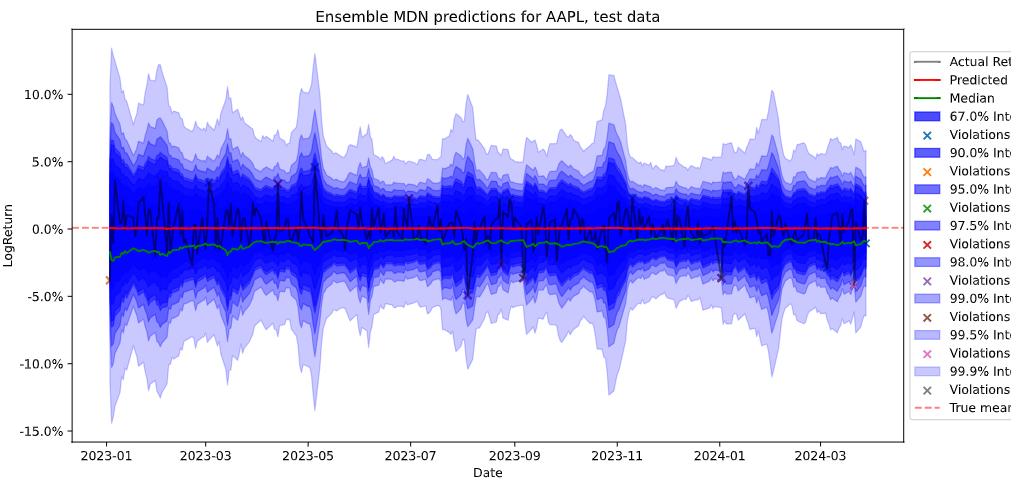
\includegraphics[width=\linewidth, height=5cm]{Images/Results/APPL_aleatoric_uncertainty_time_series_example_1.png}
        \caption{Time series of aleatoric (data-driven) uncertainty  over a 150-day rolling horizon.}
        \label{fig:aleatoric_uncertainty_time_series}
    \end{subfigure}
    \hfill
    \begin{subfigure}[b]{0.49\textwidth}
        \centering
        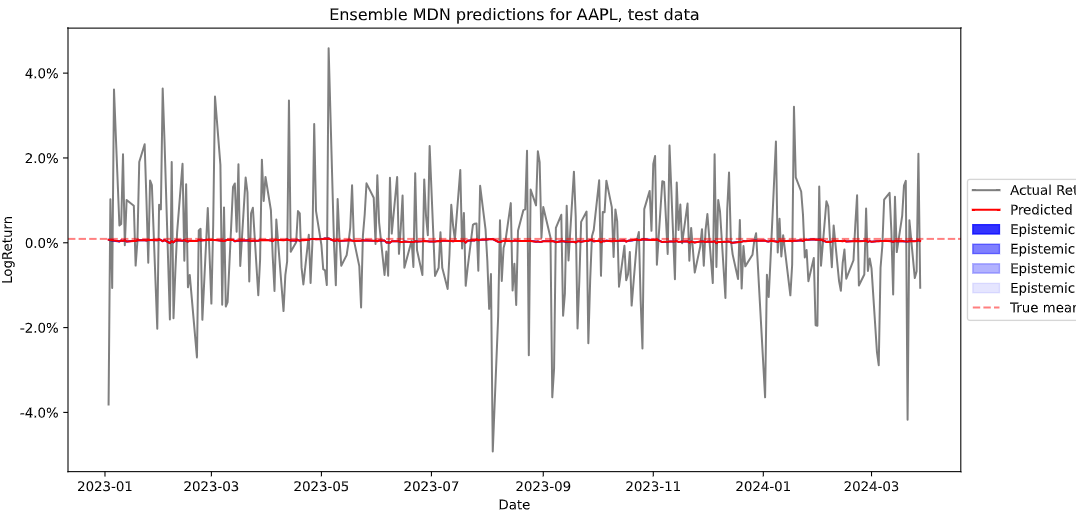
\includegraphics[width=\linewidth, height=5cm]{Images/Results/APPL_epistemic_uncertainty_time_series_example_1.png}
        \caption{Time series of epistemic (model-driven) uncertainty  over a 150-day rolling horizon.}
        \label{fig:epistemic_uncertainty_time_series}
    \end{subfigure}
    \caption{Rolling one-day-ahead predictive uncertainty decomposition over time for APPL and WMT.}
    \label{fig:uncertainty_time_series_decomposition}
\end{figure}

The average uncertainty decomposition across all models and stocks are reported in Table \ref{table:uncertainty_decomposition_proposed_models}. This shows that the total uncertainty is largely aleatoric uncertainty, with low epistemic uncertainty across assets. 


\begin{table}[H]
    \centering
    \caption[Uncertainty Decomposition into Aleatoric and Epistemic Components for Proposed Models Across Stocks]{Uncertainty Decomposition into Aleatoric and Epistemic Components for Proposed Models Across Stocks}
    \label{table:uncertainty_decomposition_proposed_models}
    \begin{tabular}{
        p{0.24\textwidth}  % Model column
        >{\centering\arraybackslash}p{0.23\textwidth}
        >{\centering\arraybackslash}p{0.23\textwidth}
        >{\centering\arraybackslash}p{0.23\textwidth}
    }
        \toprule
        \textbf{Model} & \textbf{Aleatoric Uncertainty (Avg.)} & \textbf{Epistemic Uncertainty (Avg.)} & \textbf{Total Uncertainty (Avg.)} \\
        \midrule
        LSTM-MDN-RV & $2.0 \times 10^-4$ & - & - \\
        LSTM-MDN-IV & $2.1 \times 10^-4$ & - & - \\
        LSTM-MDN-RV-IV & $2.2 \times 10^-4$ & - & - \\
        Transformer-MDN-RV & $2.0 \times 10^-4$ & $1.4 \times 10^-9$ & $2.0 \times 10^-4$ \\
        Transformer-MDN-IV & $4.6 \times 10^-4$ & $1.6 \times 10^-9$ & $4.6 \times 10^-4$ \\
        Transformer-MDN-RV-IV & $2.8 \times 10^-4$ & $2.2 \times 10^-9$ & $2.8 \times 10^-4$ \\
        \bottomrule
    \end{tabular}
\end{table}


%COULD INCLUDE SOMETHING ABOUT THE VARIATION IN DISTRIBUTION FOR THE DIFFERENT MODELS


% COULD ALSO INCLUDE SOME DISTRIBUTION OVER TIME WITH THE WEIGHTS FOR EACH DISTRIBUTION FOR ALL THE MODELS IN THE ENSEMBLE, SHOWNG THE MEAN AND DEVIATIONS, SO WE CAN SEE HOW UNCERTAIN THE MODEL IS ON WHAT IS THE CORRECT MODEL WEIGHTS

% ==================== Economic Test Results ==================== %
\subsection{Economic Test Results}
\label{sec:economic_test_results}




% ==================== Feature Importance and XAI ==================== %
\subsection{Feature Importance and XAI}
\label{sec:feature_importance_xai}
\begin{itemize}
    \item Feature importance
    \begin{itemize}
        \item SHAP (SHapley Additive exPlanations)
    \end{itemize}
    \item Attention Visualization (for Transformers or Attention-based LSTMs)
    
\end{itemize}